%:
% Typeset with XeLaTeX
% Allows use of system fonts rather than just LaTeX's ones
% NOTE - if you use TeXShop and Bibdesk (Mac), can complete citations
%  - open your .bib file, type \citep{xx... and then F5 or Option-Escape
\documentclass[12pt]{article} % 12pt with Minion Pro
% for NIH - print this PDF at 104% to be sure it's no more than 15 characters
%  per inch and no less than 6 lines per inch (with Minion Pro 12pt)
\usepackage{geometry} % set page layout
\usepackage{bbm}

% this gives reasonable margins for NIH forms after the 104% print
\geometry{letterpaper, margin=1in} % 1 inch margins
\usepackage[xetex]{graphicx} % allows us to manipulate graphics.
% Replace option [] with pdftex if you don't use Xe(La)TeX
\usepackage{color}
%\usepackage{hyperref}
\usepackage{epstopdf} % automatic conversion of eps to pdf 
\usepackage{amsmath, amssymb} % Better maths support & more symbols
\usepackage{enumitem}[shortlabels] % control over indentation for enumerate etc.
\usepackage{textcomp} % provide lots of new symbols - see textcomp.pdf
%\usepackage{enumerate}% http://ctan.org/pkg/enumerate
% line spacing: \doublespacing, \onehalfspacing, \singlespacing
\usepackage{setspace}
\singlespacing
% allows text flowing around figs
% use \begin{wrapfigure}{x}{width} where x = r(ight) or l(eft)
\usepackage{wrapfig}
\usepackage{float}
\usepackage{floatflt}
\usepackage{relsize}
\usepackage[parfill]{parskip} % don't indent new paragraphs
%\usepackage{flafter}  % Don't place figs & tables before their definition 
\usepackage{verbatim} % allows \begin and \end{comment} regions
\usepackage{bibentry} % for no bibliography
\usepackage{booktabs} % makes tables look good
\usepackage{bm}  % Define \bm{} to use bold math fonts
% linenumbers in L margin, start & end with \linenumbers \nolinenumbers,
\usepackage{lineno} % use option [modulo] for steps of 5
\usepackage[auth-sc]{authblk} % authors & institutions - see authblk.pdf
\renewcommand\Authands{ and } % separates the last 2 authors in the list
% control how captions look; here, use small font and indent both margins by 20pt
% margin option doesn't seem to work with wrapfig
\usepackage[margin=0pt,size=footnotesize, labelfont=bf, labelsep=colon]{caption}

\usepackage{sidecap}
\usepackage{algorithm}
\usepackage{algpseudocode}
%\usepackage[capbesideposition=outside,capbesidesep=quad]{floatrow}

 % Nice tables
\usepackage{colortbl}% http://ctan.org/pkg/colortbl
\usepackage{xcolor}% http://ctan.org/pkg/xcolor
\colorlet{tablerowcolor}{gray!10} % Table row separator colour = 10% gray
\newcommand{\rowcol}{\rowcolor{tablerowcolor}}
 
\usepackage{multicol}


\usepackage{gensymb} % for degree and SI units>
 
%:FONT
% If you don't want to use system fonts, replace from here to 'Citation style' with \usepackage{Palatino} or similar
\usepackage[no-math]{fontspec} % 'no-math' = keep computer modern for math fonts unless you say differently below
\usepackage{xunicode} % needed by XeTeX for handling all the system fonts nicely
\usepackage[no-sscript]{xltxtra} 
%\setmonofont[Scale=0.8]{Lucida Sans} % typeface for \tt commands
%\setsansfont[BoldFont={Lucida Sans Demibold Roman}, ItalicFont={Lucida Sans Italic}]{Lucida Sans} %my choice of sans-serif font
\defaultfontfeatures{Mapping=tex-text} % convert LaTeX specials (``quotes'' --- dashes etc.) to unicode, to preserve them
%\setmainfont[BoldFont={Minion Pro Bold.otf}, ItalicFont={Minion Pro Italic.otf}]{Minion Pro Reg.otf} %%% for overleaf
%\setmainfont{Utopia Std}
%\setmainfont{Palatino Linotype}
%\setmainfont{Minion Pro} % <------ causes error on windows
\setmainfont{Times New Roman}
%:CITATION STYLE
% natbib package: square,curly, angle(brackets)
% colon (default), comma (to separate multiple citations)
% authoryear (default),numbers (citations style)
% super (for superscripted numerical citations, as in Nature)
% sort (orders multiple cites into order of appearance in ref list, or year of pub if authoryear)
% sort&compress: as sort, + multiple citations compressed (as 3-6, 15)
\usepackage[numbers,super,sort&compress]{natbib}
\usepackage{hyperref}
\hypersetup{
%allbordercolors = {white},
allbordercolors = {white}
}


%:NUMBERING STYLE FOR BIBLIOGRAPHY
% (e.g, here it will be 1. and not [1] as in standard LaTeX)
\makeatletter
\renewcommand\@biblabel[1]{#1.}
\makeatother

%:SHORTCUT COMMANDS
% Maths
\newcommand{\ddt}[1]{\ensuremath{\frac{{\rm d}#1}{{\rm d}t}}}  % d/dt
\newcommand{\dd}[2]{\ensuremath{\frac{{\rm d}#1}{{\rm d}#2}}} % dy by dx  - \dd{y}{x}
\newcommand{\ddsq}[2]{\ensuremath{\frac{{\rm d}^2#1}{{\rm d}#2^2}}} % second deriv
\newcommand{\pp}[2]{\ensuremath{\frac{\partial #1}{\partial #2}}} % partial \pp{y}{x}
\newcommand{\ppsq}[2]{\ensuremath{\frac{\partial^2 #1}{\partial {#2}^2}}}
\newcommand{\scinot}[2]{\ensuremath{#1 \times 10^{#2}$}}
\newcommand{\superscript}[1]{\ensuremath{^{\textrm{#1}}}} %normal (non-math) font for super/subscripts in text
\newcommand{\subscript}[1]{\ensuremath{_{\textrm{#1}}}}
\newcommand{\posi}{\ensuremath{^+}}
\newcommand{\nega}{\ensuremath{^-}}
% Text
\newcommand{\khi}{\ensuremath{\text{Ki67}^\text{hi}}~}
\newcommand{\klo}{\ensuremath{\text{Ki67}^\text{lo}}~}
\newcommand{\poseight}{\ensuremath{\text{CD8}^+}}
\newcommand{\posfour}{\ensuremath{\text{CD4}^+}}
\newcommand{\trm}{T$_\text{RM}$}
\newcommand{\tcm}{T$_\text{CM}$}
\newcommand{\tem}{T$_\text{EM}$}
\newcommand{\treg}{T$_\text{reg}$}
\newcommand{\tvm}{T$_\text{VM}$}

\newcommand{\tighten}{\vspace{-0.35cm}}
\newcommand{\tightenabit}{\vspace{-0.15cm}}

\newcommand{\ie}{\textit{i.e.}~}
\newcommand{\etal}{\textit{et al}}

% how to highlight my name in reference lists - choose one of the following
\newcommand{\myemphasis}[1]{\textbf{\underline{#1}}} 
%\newcommand{\myemphasis}[1]{\textsc{#1}} % small caps
%\newcommand{\myemphasis}[1]{\textbf{#1}} % bold

% how you want volume of journals to look
\newcommand{\volume}[1]{\textbf{#1}} 
\newcommand{\bi}{\begin{itemize}}
\newcommand{\ei}{\end{itemize}}

% Formatting
\newcommand{\para}[1]{\vspace*{-4.5mm}\paragraph{#1}}
% Editing

\usepackage{color}
\definecolor{mygray}{rgb}{0.2, 0.2, 0.2}
\newcommand{\red}[1]{{\color{red}{#1}}}
\newcommand{\blue}[1]{{\color{magenta}{#1}}}
\newcommand{\cyan}[1]{{\color{cyan}{#1}}}
\newcommand{\gray}[1]{{\color{mygray}{#1}}}
% Standard stuff
\newcommand{\be}{\begin{equation}}
\newcommand{\ee}{\end{equation}}
\newcommand{\bea}{\begin{eqnarray}}
\newcommand{\eea}{\end{eqnarray}}


\renewcommand\refname{Cited literature}
%% \begin{graybox} text \end{graybox} for text with a background colour
%\definecolor{MyGray}{rgb}{0.96,0.97,0.98}
%\definecolor{MyGray}{rgb}{0.96,0.90,0.98}
%\makeatletter\newenvironment{graybox}{%
%   \begin{lrbox}
%   {\@tempboxa}\begin{minipage}[r]{0.98\columnwidth}}{\end{minipage}\end{lrbox}%
%   \colorbox{MyGray}{\usebox{\@tempboxa}}
%}\makeatother

%%%%%%%%%%%%%%%%%%%%%%%%%%
\usepackage{empheq}
\usepackage[most]{tcolorbox}

\newtcbox{\mymath}[1][]{%
    nobeforeafter, math upper, tcbox raise base,
    enhanced, colframe=blue!30!black,
    colback=blue!30, boxrule=0.65pt,
    #1}


\usepackage{url}\newcommand\hi{$^\text{high}$}
\newcommand\lo{$^\text{low}$}


% diagrams in latex
\usepackage{tikz}
\usetikzlibrary{shapes.geometric, arrows}
\tikzstyle{box1} = [rectangle, rounded corners, minimum width=2cm, minimum height=1cm, text centered, draw=black, fill=green!60]
\tikzstyle{box2} = [rectangle, rounded corners, minimum width=2cm, minimum height=1cm, text centered, draw=black, fill=green!30]
\tikzstyle{box3} = [rectangle, rounded corners, minimum width=2cm, minimum height=1cm, text centered, draw=black, fill=yellow!60]
\tikzstyle{box4} = [rectangle, rounded corners, minimum width=2cm, minimum height=1cm, text centered, draw=black, fill=blue!30]
\tikzstyle{box5} = [rectangle, rounded corners, minimum width=2cm, minimum height=1cm, text centered, draw=black, fill=blue!60]


\usepackage{fancyhdr}


%\renewcommand{\thesection}{\Alph{section}}
%\renewcommand{\thesubsection}{\thesection\Alph{subsection}}

%%%%%%%%%%%%%%%%%%%%%%%%%%

\begin{document}
\title{Generative Language Modeling for Bayesian Inference on Dynamical Data}
\author[1]{Jun Won Park}
\author[1]{Sanket Rane}
\affil[1]{Irving Institute for Cancer Dynamics, Columbia University, New York, NY, USA}
%\setcounter{Maxaffil}{0}

\maketitle
%
%\newpage
%
%\section*{Contents}
%
%\begin{enumerate}
%\item Introduction
%\vspace{6mm}
%\item Methods
%\vspace{6mm}
%\item Results
%\vspace{6mm}
%\item Discussion
%\end{enumerate}
%
%\newpage
%
\begin{abstract}
% -Likelihood free parameter estimation.
% -Reliance on summary statistics – issues with that.
% -Multidimensional data – ill posed inverse problems.
% -Use of generative models to convert inverse problem into a (machine) learning problem
We introduce viaABC (Variational Inference Assisted Approximate Bayesian Computation), a novel likelihood-free parameter estimation framework that integrates Approximate Bayesian Computation (ABC) with Variational Autoencoders (VAEs). Traditional ABC methods rely on carefully chosen summary statistics, which can be challenging to define in high-dimensional settings, often leading to ill-posed inverse problems. viaABC mitigates this limitation by leveraging the representational power of VAE, a generative model, to learn a structured manifold representation of data beyond the constraints of Euclidean space. This approach is particularly advantageous for complex datasets, including hierarchical time series, spatial, spatio-temporal, and stochastic dynamical systems, enabling more robust and scalable parameter inference in likelihood-free settings.
\end{abstract}

\section{Introduction}
% Need for a new approach
% Blurb about inverse problems, Bayesian approaches to solve inverse problems, their shortcom-
% ings.

% ABC for likelihood free inference, summary statistics are NOT always the answer, discuss con-
% temporary alternatives for summary statistics.

% Multidimensional data is a norm in biology now, how to handle large scale data or generate
% summary statistics from them?

% Our solution is to perform inference in the latent space – follows manifold hypothesis, which posits
% that high-dimensional data often lie in low dimensional manifolds within the high-dimensional
% data. Better representation to perform causal inference on dynamical data.


Inference drawn from mathematical modeling of biological data hinges on accurately identifying model parameters and capturing uncertainty in their estimation.
Mechanistic models predict causal structure and dynamical models predict the evolution of a system over time. These models are often expressed as ordinary differential equations (ODEs) or partial differential equations (PDEs), which can be challenging to solve analytically. As a result, numerical methods are frequently employed to simulate the model's behavior, generating synthetic data that can be compared to experimental observations. This process is known as inverse modeling, where the goal is to infer the model parameters from observed data.
Mechanistic inference is essential for understanding phenomena across various scientific disciplines, as it enables the mathematical modeling of dynamical systems and the extraction of their underlying parameters. Therefore, accurately inferring model parameters, denoted as $\theta$, from experimentally observed data, $y^{\text{obs}}$, is crucial. In the Bayesian framework, this involves determining the posterior distribution
$$\pi(\theta | y^{obs}) \propto f(y^{obs} | \theta)\cdot \pi(\theta) $$
of the parameters from the data by calculating the likelihood $f(y^{obs} | \theta)$ of such observations under the model with given parameter values. However, deriving the likelihood function theoretically is often intractable, computationally expensive, or too complex for direct optimization. Approximate Bayesian Computation (ABC) was introduced as an alternative framework for approximating posterior distributions when traditional likelihood-based methods are impractical \citep{tavare1997inferring}. This approach either employs summary statistics to represent both simulated and observed data using a distance metric to gauge their similarity in the case high-dimensional data or it directly compares the raw simulated and observed datasets. In both cases, ABC aims to identify the parameter values that minimize the discrepancy between the two. Numerous variants of the ABC algorithm have since been developed, including ABC Monte Carlo Markov Chain \citep{marjoram2003markov}, ABC Sequential Monte Carlo \citep{toni2009approximate}, and ABC Population Monte Carlo \citep{robert2008adaptivity}, each of which has demonstrated effectiveness across a wide range of scientific disciplines.

Despite their success, the accuracy and efficiency of existing Approximate Bayesian Computation (ABC) methods heavily depend on the selection of hyperparameters, including summary statistics and distance metrics, which are often data-dependent and require extensive tuning. In particular, reducing data to a few informative summary statistics is a critical step that directly influences the accuracy of the inference. The choice of these statistics must be made carefully, as it determines the quality of the representation and, consequently, the reliability of the results \citep{aakesson2021convolutional}. This challenge is especially pronounced in biological applications, where data is inherently high-dimensional. As the dimensionality increases, identifying a compact yet informative set of summary statistics becomes impractical. Additionally, the choice of distance metric, including how to weight each statistics, also influences the accuracy of the parameter estimation.

To address these limitations, we introduce viaABC, a novel statistical inference framework that leverages techniques from computer vision and natural language processing to enhance approximate posterior inference in mechanistic modeling. By learning a structured representation of data through variational inference, viaABC eliminates the reliance on manually selected summary statistics and distance metrics, thereby improving both the accuracy and robustness of ABC-based inference. Based on the manifold hypothesis that high-dimensional data often reside near low-dimensional manifolds \citep{fefferman2016testing}, viaABC facilitates inference on complex, high-dimensional datasets, addressing challenges typically encountered in such analyses. 


The contributions of this paper can be summarize as follows:
\begin{enumerate}
\item \textit{Generality}: VAE can learn a dense, vector representation of data, eliminating the need for using summary statistic to represent data
\item \textit{Sample efficiency}: The proposed framework is empirically shown to require less number of simulations than previous methods
\item \textit{Noise modeling}: Our framework is more flexible and robust towards experimental and biological noises
\end{enumerate}

Our work will primarily focus on multivariate time-series data. Our method employs self-supervised pre-training on simulated multivariate time-series data. During pre-training, the model captures temporal and cross-channel dependencies, constructing a latent distribution for each time step. This process yields an entangled representation of the time-series data. The pre-trained model then generates latent representations for simulated data, which are subsequently compared to the representation of $y^{obs}$ for parameter inference using sequential ABC.

\section*{Related Work}

\para{ABC}
This section provides a comprehensive review and development of the theoretical foundations of Approximate Bayesian Computation (ABC), with a particular focus on its applications to dynamical systems and statistical parameter inference before introducing the variational inference approach in the context of ABC. 

\para{ABC Rejection}
Approximate Bayesian Computation (ABC) rejection is a method for parameter inference when likelihoods are intractable or computationally expensive to evaluate \citep{tavare1997inferring}. The process begins by defining prior distributions for the parameters, a distance metric, and summary statistics. Common distance metrics include L1 and L2 distances, while statistics often include the mean, variance, or combinations of moments. A parameter set is then sampled from the prior distributions and passed through a predefined simulator, a mathematical model describing the system's dynamics. The resulting statistics are computed and compared to those from the observed data. If the distance between the simulated and observed statistics falls within an acceptance threshold, the parameter set is retained for the approximate posterior; otherwise, it is rejected.

\para{Sequential ABC}
Approximate Bayesian Computation (ABC) rejection sampling relies on several hyperparameters, including the rejection threshold and the choice of distance metric for comparing simulated and observed data. A small rejection threshold typically results in a low acceptance rate, leading to high computational costs, especially when the prior distribution differs significantly from the posterior \citep{toni2009approximate}. To address this, ABC Population Monte Carlo (ABC-PMC) and ABC Sequential Monte Carlo (ABC-SMC) were introduced, which the idea is to begin with a large threshold and iteratively reduce it. In each iteration, samples, referred to as particles, are drawn from the approximate posterior of the previous iteration, iteratively refining the shape of the posterior distribution and improving sampling efficiency. The key distinction between ABC-PMC and ABC-SMC lies in the choice of the perturbation kernel. ABC-SMC assumes no explicit perturbation kernel, though prior studies have seen success using a uniform distribution. In contrast, ABC-PMC utilizes a multivariate normal distribution for perturbation, allowing for smoother updates and potentially more efficient exploration of the posterior space.

% \subsection{Self-supervised Learning (SSL)}
% Self-supervised learning (SSL) has achieved remarkable success in natural language processing and computer vision, with applications extending beyond text and images to modalities such as video, audio, and time series \citep{balestriero2023cookbook}. Broadly, SSL can be categorized into contrastive learning and masked learning.

% \subsection*{Contrastive Representation Learning}
% The core idea of contrastive loss is to generate two augmented versions of a given input: a positive sample that is similar to the input and a negative sample that is dissimilar. The objective is to encourage similar representations to cluster together while pushing dissimilar ones apart.\\
% PLACEHOLDER FOR CONTRASTIVE LOSS APPROACHES IN TIME-SERIES 

\para{Masked Modeling}
Self-supervised learning (SSL) has demonstrated remarkable success in natural language processing and computer vision, with its applications extending beyond text and images to modalities such as video, audio, and time series \citep{balestriero2023cookbook}. In this publication, we explore the masked modeling approach, a prominent self-supervised learning technique.

The masked modeling approach learns useful representations by masking parts of the input and reconstructing them using the unmasked portions. This technique has been successful in natural language processing, as demonstrated by masked language modeling in BERT, where some tokens are randomly masked, and the model predicts the missing tokens based on the surrounding context \citep{devlin2019bert}. In computer vision, an image is divided into patches, with some randomly masked, and the model reconstructs the original image using the remaining patches \citep{he2022masked}.

There are several variations of masked modeling. One approach masks portions of the input before passing it through the model, as seen in BERT, while another applies masking to the output of the encoder, as used in MAE. The optimal masking ratio varies depending on the application: in BERT, an effective masking ratio is approximately 15\%, whereas in MAE, it reaches as high as 75\% \citep{yao2022masked}.

Masked modeling has been adopted into time-series domain for time-series forecasting like TiMAE and TimeMAE \citep{li2023ti}\citep{cheng2023timemae}. By reconstructing the missing time-stamps from partially masked inputs, the model gathers contextual information to predict the missing regions, enhancing the model's understanding of complex interaction relationships between different dimensions.

\para{Varitional Autoencoder}
%TODO: fix this 
Variational inference (VI) has been proposed as a machine learning approach to approximate intractable probability densities, as an alternative method to Markov Chain Monte Carlo (MCMC) sampling. \citep{jordan1999introduction}\citep{Blei_2017}. There are numerous advantages to variational inference: variational inference is typically much faster especially for high-dimensional data and is much easier to scale to large data \citep{Blei_2017}.

Variational autoencoders (VAEs) are deep latent variable models that leverage variational inference for approximate posterior inference. When a neural network is used for the recognition model, an approximation to the intractable true posterior, i.e. $q_{\phi}(z|x)$, we call it a variational auto-encoder \citep{kingma2013auto}. 

Variational autoencoder consists of a probabilistic encoder $q_{\phi}(z|x)$ and a probabilistic decoder $p_{\theta}(x|z)$. 

%Under this framework, one typically takes the reconstructions as deterministic, corresponding to the mean of the decoder, namely $g_{\theta}(z) := E_{p_{\theta}(x|z)}[X]$.


% Given a dataset $\textbf{X} = \{x^{(i)}\}_{i=1}^{N}$ consisting of $N$ i.i.d. samples of a continuous or discrete variable $x$, we assume that the data are generated by an underlying random process involving an unobserved continuous latent variable $z$ \citep{kingma2013auto}. The generative process follows two steps:
% \begin{enumerate}
% \item A latent variable $z^{(i)}$ is drawn from a prior distribution $p_{\theta^*}(z)$.
% \item A corresponding observation $x^{(i)}$ is sampled from a conditional distribution $p_{\theta^*}(x \mid z)$.
% \end{enumerate}



% We assume that both the prior $p_{\theta^*}(z)$ and the likelihood $p_{\theta^*}(x \mid z)$ belong to parametric families of distributions $p_{\theta}(z)$ and $p_{\theta}(x \mid z)$, respectively, and that their probability density functions are differentiable with respect to both $\theta$ and $z$. However, much of this process remains hidden: the true parameters $\theta^*$, as well as the values of the latent variables $z^{(i)}$, are unknown. \textbf{PARAPHRASE THIS AND CITE KINGMA}

\newpage
\subsection*{Cosine similarity of the latent variables as an acceptance criterion}




there is relationship between data points that can inform on model parameters. that information could be projected to latent manifolds to either lower or higher dimensions. 
We exploit deep learning to generate latent representations of the data, which can be used as summary statistics in a Bayesian framework.
%The latent representation is learned from simulated data, and we use it to compare with the observed data. 
This approach allows us to bypass the need for manually selecting summary statistics, which can be challenging in high-dimensional settings. 
we can fit models in the real space and it will work sometimes/often but we can learn crucial insights about these relationships by learning the latent representation.

\blue{simulation based inference}.

\para{Training:}
Suppose we have a mathematical model or data-generating process, denoted as \( f \), which maps a \( k \)-dimensional parameter vector to a \( d \)-dimensional multivariate time series:  

$$
f(\theta) = \{X_t\}_{t=1}^T, \quad \theta \in \mathbb{R}^k.
$$  

To construct a training data set, we use Latin hypercube sampling (LHS), a commonly used sampling technique in monte carlo simulations, to generate \( N \)  parameter sets, each of which is used to simulate an associated multivariate time series \citep{}. Specifically, we denote the \( i \)-th simulated time series as  

$$
\{X_{t}^{(i)}\}_{t=1}^T, \quad X_t^{(i)} \in \mathbb{R}^d,
$$  

where each sample represents a realization of the underlying process. This procedure yields a dataset consisting of \( N \) multivariate time series samples. To facilitate the study of the model dynamics across a diverse range of parameter configurations, we employ Latin hypercube sampling based on the reasoning that a well-distributed exploration of the parameter sample space is potentially better, thus mitigating the risk of overfitting to any particular mode\citep{mckay2000comparison}. 

During training, Gaussian noise \( \epsilon \) is dynamically injected at each time step such that  

$$
\tilde{X_t} = X_t + \epsilon, \quad \epsilon \sim \mathcal{N}(0, \sigma^2).
$$  

The noise should be dimension-scale dependent. The variational autoencoder (VAE) is trained using noise-injected time series data as input, learning to reconstruct the original denoised data. The purpose of this is to allow the model to learn a representation that understands biological variation. In biology, observational data incorporate both biological variation and experimental variation. By dynamically injecting noise during pre-training, we

In addition to minimizing reconstruction loss, the VAE also minimizes Kullback-Leibler (KL) divergence to regularize the latent space and encourage a structured representation. In this study, we enforce a Gaussian prior on the latent space.

\textbf{Objective function}: Like any other VAE, the objective function optimizes the Evidence Lower Bound (ELBO). We define the loss function as a combination of reconstruction loss and KL divergence, applied at each time step. Since we employ the VAE in a time-step-wise manner, the loss function for each time step t consists of the reconstruction loss and the Gaussian KL divergence loss:

$$L_t = \frac{1}{2}MSE(x_t, \hat x_t) + \beta D_{KL}(q_{\phi}(z_{t}|x_{t})||p_{\theta}(z_{t}))$$

Aggregating the losses over the entire time sequence, the total loss is given by:

\begin{align*}
L &= \frac{1}{T}\sum_{t=1}^{T} L_t\\
&= \frac{1}{T}(\frac{1}{2N \cdot D}\sum_{i=1}^{N}\sum_{j=1}^d(x_{t,j}^{(i)} - \hat x_{t,j}^{(i)})^2 + \beta D_{KL}(q_{\phi}(z_{t}|x_{t})||p_{\theta}(z_{t})))
\end{align*}

where $\beta$ is a hyper-parameter that balances the trade-off between latent channel capacity and independence constraints with reconstruction accuracy\citep{higgins2017beta}.

%Notation: $X^{(i)}_{t,j}$ denotes a point in the i-th sample, at time-stamp t and in the d-th dimension.\\

%Per time-stamp: $$L_{t} = \frac{1}{2N \cdot d}\sum_{i=1}^{N}\sum_{j=1}^d(x_{t,j}^{(i)} - \hat x_{t,j}^{(i)})^2 + \beta D_{KL}(q_{\phi}(z_{t}|x_{t})||p_{\theta}(z_{t}))$$
%
%$$L = \frac{1}{2N \cdot T \cdot d}\sum_{i=1}^{N}\sum_{t=1}^{T}\sum_{j=1}^d(x_{t,j}^{(i)} - \hat x_{t,j}^{(i)})^2 + \frac{\beta}{T}\sum_{t=1}^{T}D_{KL}(q_{\phi}(z_{t}|x_{t})||p_{\theta}(z_{t}))$$

\textbf{Scaling}: In biological data, multivariate time series often exhibit heterogeneous magnitudes, with each dimension varying significantly in scale. This variation presents optimization challenges for deep learning models, making normalization a crucial pre-processing step. In the case of TSMVAE, the goal of normalization is to ensure that values are scaled appropriately for deep learning training. This helps prevent issues such as vanishing or exploding gradients and mitigates the risk of the model disproportionately focusing on reconstructing one dimension while neglecting others, which could lead to under-fitting.

A widely used normalization approach involves applying an affine transformation to the time series, i.e.. $\tilde{x} = {(x_i - m)}/{s}$ \citep{rabanser2020effectiveness}\citep{ansari2024chronos}. Different choices of $m$ and $s$ result in  various well-known normalization techniques such as mean scaling, standard scaling, and min-max scaling.

In our study, we adopt mean scaling as the normalization technique, as it has demonstrated effectiveness in deep learning models frequently applied to practical time-series tasks \citep{salinas2020deepar}\citep{rabanser2020effectiveness} \citep{ansari2024chronos}. Mean scaling normalizes each dimension of the time series by dividing its values by the absolute mean, setting $m = 0$ and $s= \frac{1}{T} \sum_{t=1}^{T}|x_i|$ in the above affine transformation. 

Previous studies have addressed the challenge of heterogeneous magnitudes in time-series data using mean scaling, which enables deep learning models to learn scale-invariant patterns while preserving zero values \citep{ansari2024chronos}. While this property facilitates stable model training, it introduces an additional challenge in our work. Specifically, if the priors are non-informative or poorly specified, viaABC may accept particles that generate multivariate time series with differing absolute magnitudes but similar scaled representations compared to the observational data. This could lead to misleading inferences, as viaABC compares its similarity to the scaled observational data in latent space. 


\para{TSM VAE:}
We adopted the transformer-based Masked Autoencoder (MAE), originally developed for computer vision, where it employs the Vision Transformer (ViT) as the backbone model for both the encoder and decoder, to the domain of multivariate time-series data \citep{dosovitskiy2020image, he2022masked}.
While MAE has been widely employed for image representation learning, its direct application to time-series data presents challenges due to the temporal dependencies and multivariate structure inherent in such data.
To address these challenges, we formulated the Time-Series Masked Variational Autoencoder (TSMVAE), an adaptation that integrates the principles of MAE with a variational autoencoder framework tailored for time-series modeling.
%The intention of this paper is not to introduce the new model architecture.

Our model consists of an encoder that maps the observed signal into a latent representation and a decoder that reconstructs the original signal from this latent space. However, TSMVAE diverges from the original MAE in two fundamental ways to better capture the structure of multivariate time-series data:

\para{Temporal Patching}: Given a $D$-dimensional time-series, $\{X_t\}_{t=1}^{T}$, where $X_t \in \mathbb{R}^D$, TSMVAE partitions the sequence along the time axis, forming patches that correspond to different time intervals. Each patch is then projected into a higher-dimensional space via a linear transformation, facilitating the encoding of temporal dependencies.

\para{Variational Latent Space Representation}: The encoded output undergoes two additional linear transformations. The first maps the encoded representations into a predefined latent dimension, structuring the latent space effectively. The second transformation introduces variational layers, which impose a probabilistic structure on the latent variables, thereby enabling the learning of meaningful latent distributions. 

These modifications enable TSMVAE to effectively learn representations from multivariate time-series data time-stamp wise while leveraging the power of masked self-supervised learning. Figure 1 provides a high-level illustration of our proposed model. For further details on the model architecture, we refer the reader to prior work.

\begin{figure}
    \centering
    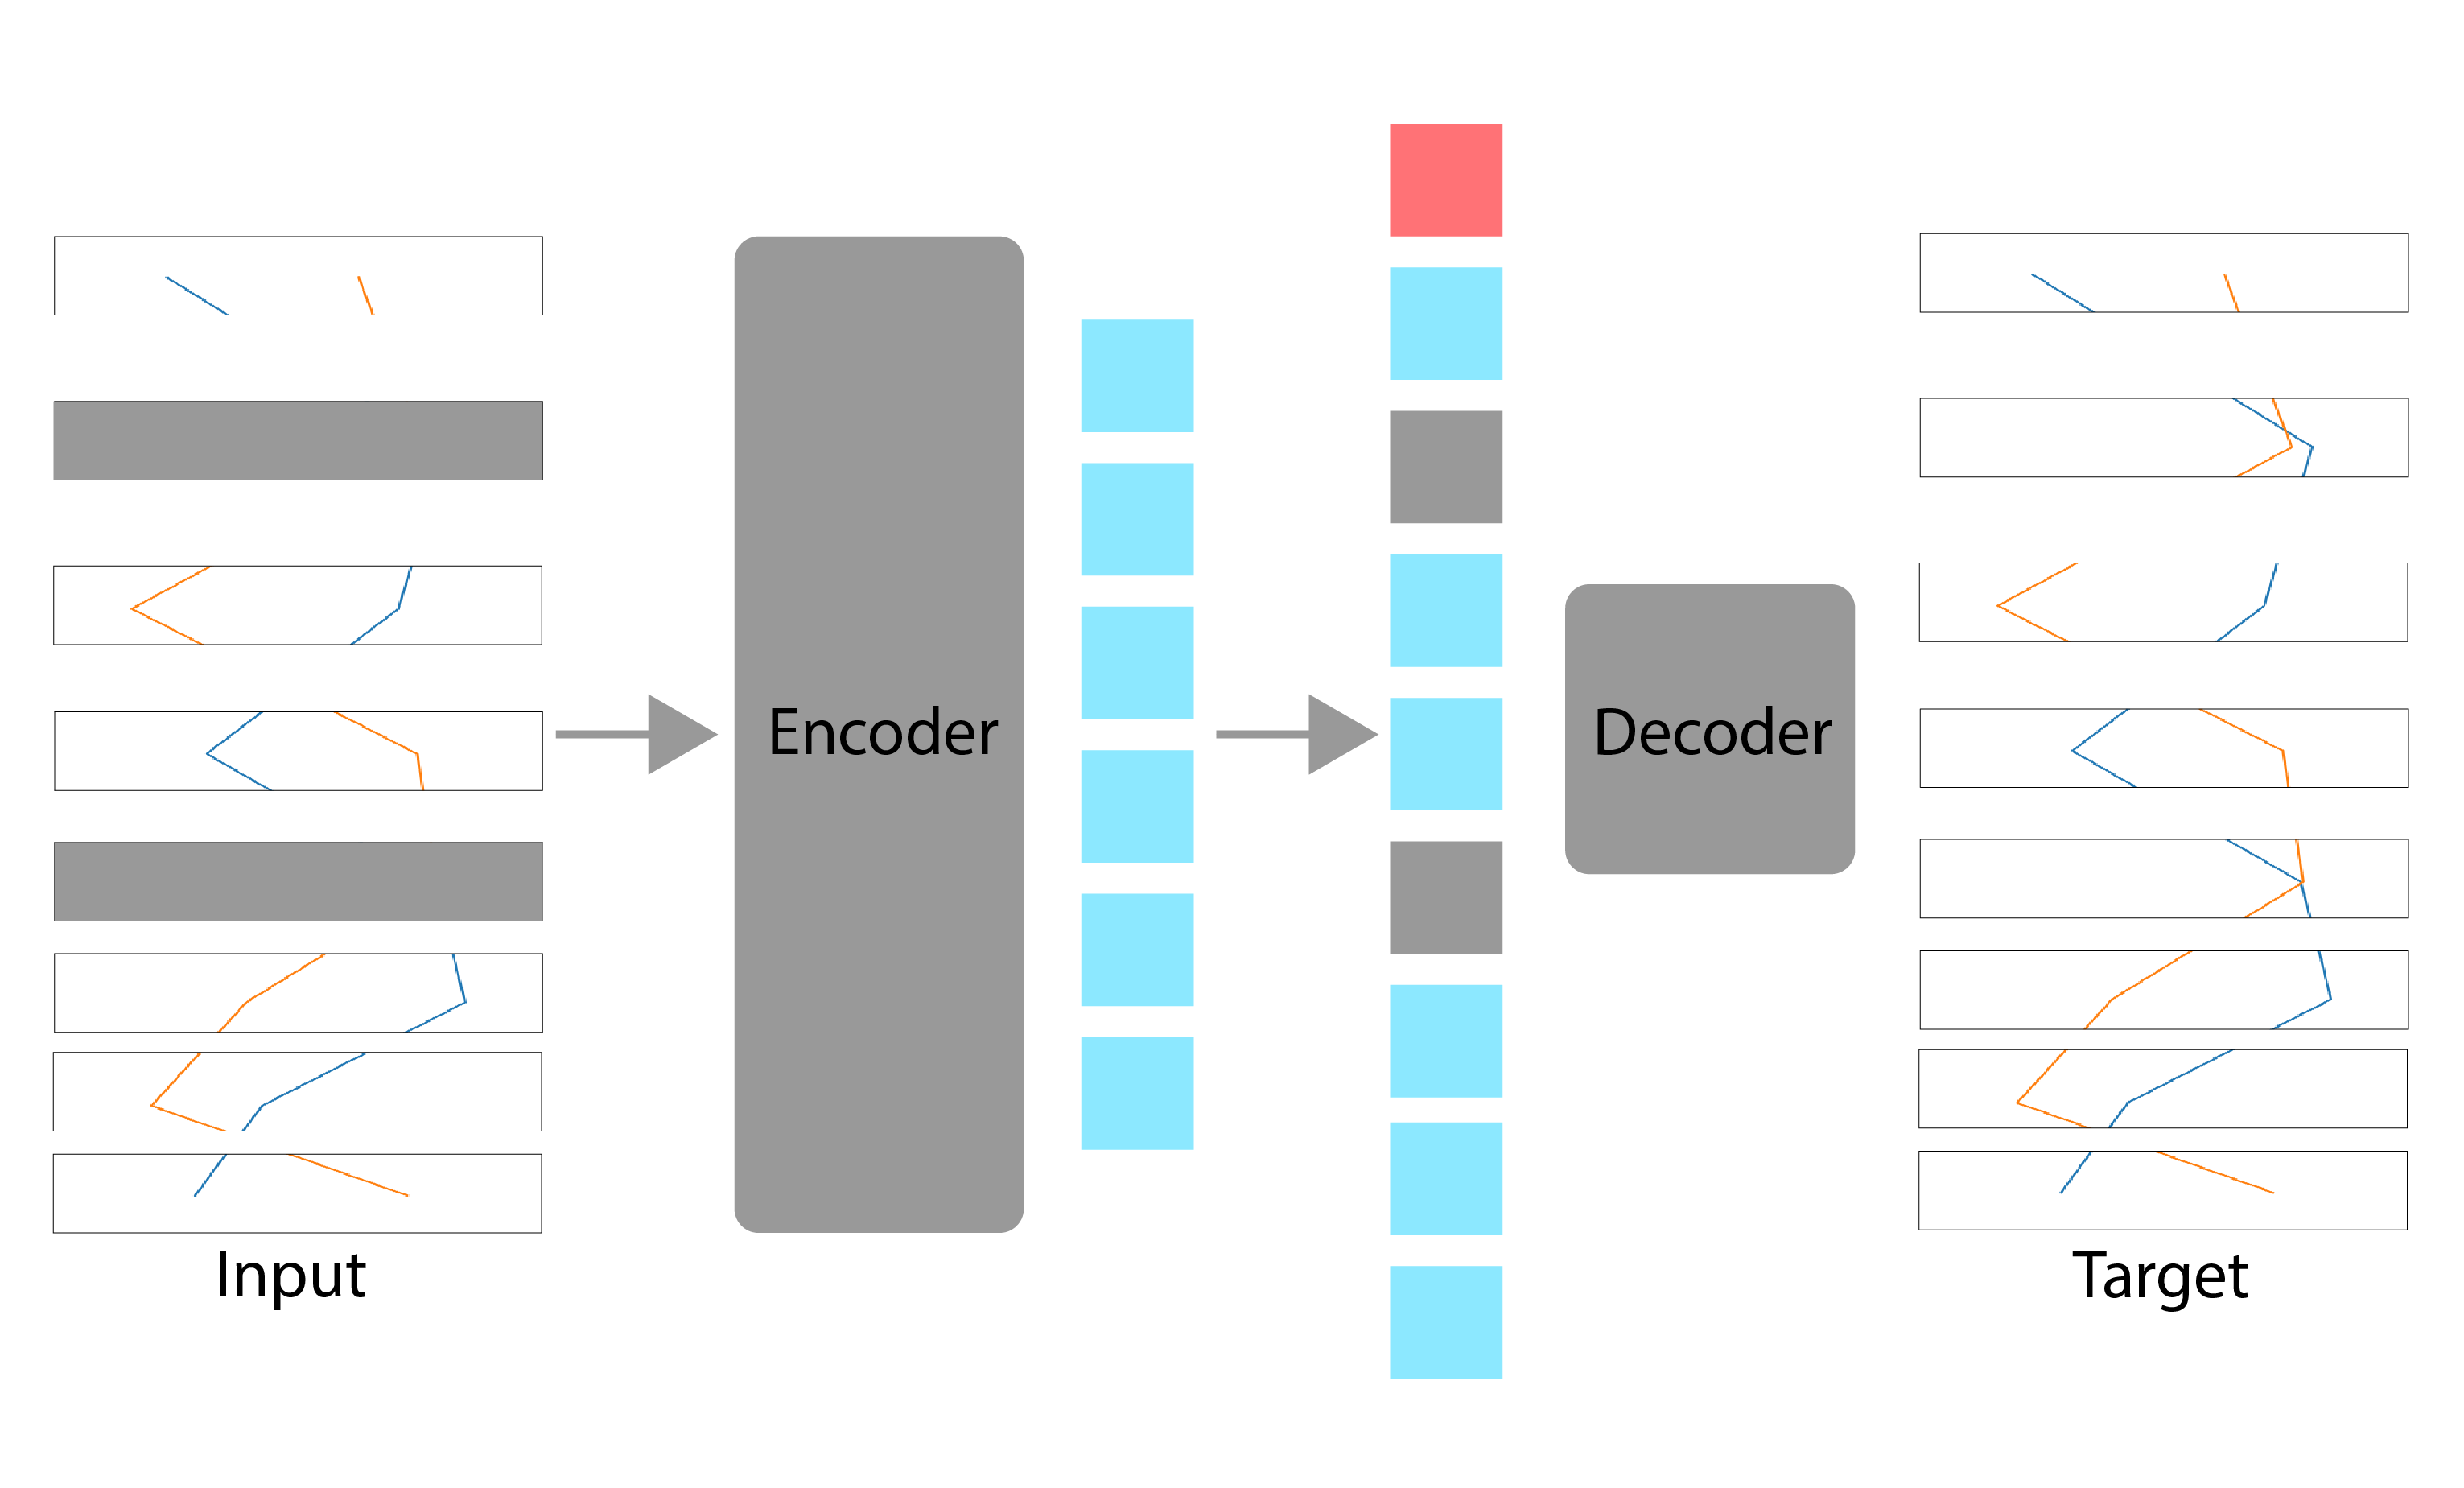
\includegraphics[width=0.75\linewidth]{figures/model_architecture.png}
    \caption{\textbf{Tokenized encoding and sequential Monte Carlo to generate posterior distribution of parameters}.
\blue{this figure will be the full schematic of VIA-ABC}. \\    
During pretraining, a random subset of temporal patches (e.g., 15\%) is masked out. The encoder is applied to the visible patches. The CLS token (red) and Mask tokens (gray) are introduced after the encoder, and the full set of encoded patches along with the mask tokens undergoes the reparametrization trick. This is then processed by a small decoder that reconstructs the original patches. After pretraining, the decoder is discarded, and the encoder is applied to uncorrupted multivariate time series (full sets of patches) for viaABC.}
    \label{fig:enter-label}
\end{figure}


%
%\subsection{Metric}
%
%\subsection*{Cosine Similarity}
%
%\subsection*{BERTScore}
%we utilize BERTScore as our distance metric to compare similarity between latent representations of observed data and simulated data. Originally developed as an automatic evaluation tool for text generation, BERTScore assesses sentence similarity by leveraging contextual embeddings \citep{zhang2019bertscore}. While models that generate both contextual embeddings and entangled latent representations typically require a pooling operation to condense these representations into a single vector, BERTScore obviates the need for pooling by directly comparing two matrices of latent representations, employing pairwise cosine similarity of latent representations of all time-stamps.
%
%\textbf{Figure 2} BERTScore for Time-series

%To address this issue, we introduce an auxiliary task linked to the CLS head token. Specifically, we incorporate a simple linear layer designed to predict the log-scaled magnitude of the absolute mean scales. This auxiliary task enables the construction of scale-variant latent representations while maintaining stable model training.

\textbf{Special Token}: The TSMVAE model has a special CLS token, which will be used to output a latent vector representation of a multi-variate time-series data. This is often known as the CLS pooling. 

%The CLS token functions as a way of pooling latent representations as well as it introduces us to predict the log-scaled

%[Need to study whether using contextual embeddings is better or CLS pooling is better]

\subsection{VIA-ABC}
Following the notation of \citep{marin2012approximate} and \citep{simola2021adaptive}, the resulting ABC posterior can be written as
$$
\pi_{\epsilon}(\theta | y_{obs}) = \int [\frac{f(y_{prop} | \theta)\pi(\theta)\mathbbm{1}_{A_{\epsilon, y_{obs}}}(y_{prop})}{\int_{A_{\epsilon, y_{obs}} \times \Theta } f(y_{prop} | \theta)\pi(\theta)dy_{prop}d\theta}]d_{y_{prop}}
$$
where $\mathbbm{1}_{A_{\epsilon, y_{obs}}}(\cdot)$ is the indicator function for the set $A_{\epsilon, y_{obs}} = \{y_{prop} | \rho (s(y_{obs}), s(y_{propr})) \leq \epsilon\}$ and $p(\cdot,\cdot)$ is the distance function and $s(\cdot)$ is the summary statistic function. 

In viaABC, we modify the set notation such that
$$A_{\epsilon, y_{obs}} = \{y_{prop} | \rho (z_{obs}, z_{prop}) \leq \epsilon\}$$
where $z_{obs}$ and $z_{prop}$ are latent representations of $y_{obs}$ and $y_{prop}$ respectively.

viaABC follows the Adaptive Approximate Bayesian Population Monte Carlo (aABC-PMC) algorithm \citep{simola2021adaptive}. However, it introduces three key modifications: 

\textbf{Distance Gauge}: Instead of comparing distances in the original data manifold using predefined summary statistics, viaABC encodes the data into latent vectors and evaluates distances within the latent space. The TSVMAE model incorporates a CLS token, which facilitates the aggregation of contextual information and enables the representation of a multivariate time series as a single vector. This vector is then compared between simulated and observational data using cosine similarity.

%Furthermore, the latent representations at each time step can be used to represent the multivariate time series as a matrix, or they can be aggregated into a vector by taking the mean. These latent representations enable the calculation of the distance between the simulated data and the observational data in the latent space.

\textbf{Initialization}: The initialization process leverages training data to accelerate convergence. In the aABC-PMC initialization, the algorithm samples $kN$ particles, then selects the top $N$ particles based on sorted distance\citep{simola2021adaptive}. In viaABC, we adapt this by calculating the distance between the observational data and all training samples, and selecting the top $N$ particles based on this distance. This modification is similar to aABC-SMC when $k = {N_{training}}/{N}$. A critical distinction is that in viaABC, the training samples are drawn using Latin Hypercube Sampling over the entire parameter domain, whereas aABC-PMC relies on pre-defined priors.

\textbf{Stoping Rule}: 
A few ideas have been introduced to determine how to stop in a sequential ABC algorithm. Ishida et al. \citep{ishida2015cosmoabc} proposed a stopping rule once the acceptance rate of the algorithm  falls below a certain threshold which is estimated based on the sequential ABC posterior distributions. Simola et. al \citep{simola2021adaptive} proposed using a stopping rule based on estimated quantile of the ABC posterior distributions where $q_t > 0.99$ and $ t \geq 3$. In our work, we adapt the stopping rule proposed by Simola et al and use $\epsilon_t < 0.01$ and $ t \geq 3$ as our stopping criterion. 0.01 is an arbitrary chosen threshold which has shown to work well in our examples.

%In the next section, we compare various pooling strategies, including CLS pooling, mean pooling, and contextual embeddings, alongside different distance metrics such as L1 distance, L2 distance, cosine similarity, and BERTScore.

% Move to appendix?
% \begin{algorithm}[H]
% \caption{ABC-PMC: ABC-Population Monte Carlo}
% \begin{algorithmic}[1]
% \State Given a decreasing sequence of tolerance thresholds $\epsilon_{1} \geqslant \cdots \geqslant \epsilon_{T}$,
% \Statex \textbf{Initialization ($t=1$):}
% \For{$i=1$ to $N$}
%     \Repeat
%         \State Sample $\theta^{(1)}_{i} \sim \pi(\theta)$
%         \State Simulate $y^* \sim f(x \mid \theta^{(1)}_{i})$
%     \Until{$\rho(y_{obs}, y^*) < \epsilon_{1}$}
%     \State Set $\omega^{(1)}_{i} = 1/N$
% \EndFor
% \Statex \textbf{Iterations ($2 \leqslant t \leqslant T$):}
% \For{$t=2$ to $T$}
%     \State Take $\tau^{2}_{t-1}$ as twice the weighted empirical variance of the $\{\theta^{(t-1)}_{i}\}_{i=1}^N$
%     \For{$i=1$ to $N$}
%         \Repeat
%             \State Sample $\theta^{*}_{i}$ from $\{\theta^{(t-1)}_{j}\}_{j=1}^{N}$ with probabilities $\{\omega^{(t-1)}_{j}\}_{j=1}^{N}$
%             \State Sample $\theta^{(t)}_{i} \mid \theta^{*}_{i} \sim \mathcal{N}(\theta^{*}_{i}, \tau^{2}_{t-1})$
%             \State Simulate $y^{**} \sim f(y \mid \theta^{(t)}_{i})$
%         \Until{$\rho(y_{obs}, y^{**}) \leqslant \epsilon_{t}$}
%         \State Set $\omega^{(t)}_{i} \propto \pi(\theta^{(t)}_{i}) / \sum_{j=1}^{N} \omega^{(t-1)}_{j} \phi\{\tau^{-1}_{t-1}(\theta^{(t)}_{i} - \theta^{(t-1)}_{j})\}$
%     \EndFor
% \EndFor
% \end{algorithmic}
% \end{algorithm}

% \begin{algorithm}[H]
% \caption{aABC-PMC: Adaptive ABC-Population Monte Carlo}
% \begin{algorithmic}[1]
% \State Given a final quantile $Q$ and an integer k,
% \Statex \textbf{Initialization ($t=1$):}
% \For{$i=1$ to $kN$}
%     \State Sample $\theta^{(1)}_{i} \sim \pi(\theta)$
%     \State Simulate $y^* \sim f(x \mid \theta^{(1)}_{i})$
%     \State Record $\rho(y_{obs}, y^*) = d_i$
% \EndFor
% \State Let $D =\{d_i\}_{i=1}^{kN}$ and reindex the sequence D in monotone increasing order
% \State Reindex the initial particles $\Theta_1 = \{\theta^{1}_{j}\}_{j=1}^{kN}$ based on D's index
% \State Set $\epsilon_1 = d_{1000}$
% \State Set initial particles to be the first N elements of $\Theta_1$, e.g. $\{\theta^{1}_{j}\}_{j=1}^{N}$

% \Statex \textbf{Iterations ($2 \leqslant t \leqslant T$):}
% \For{$t=2$ to $T$}
%     \State Take $\tau^{2}_{t-1}$ as twice the weighted empirical variance of the $\{\theta^{(t-1)}_{i}\}_{i=1}^N$
%     \For{$i=1$ to $N$}
%         \Repeat
%             \State Sample $\theta^{*}_{i}$ from $\{\theta^{(t-1)}_{j}\}_{j=1}^{N}$ with probabilities $\{\omega^{(t-1)}_{j}\}_{j=1}^{N}$
%             \State Sample $\theta^{(t)}_{i} \mid \theta^{*}_{i} \sim \mathcal{N}(\theta^{*}_{i}, \tau^{2}_{t-1})$
%             \State Simulate $y^{**} \sim f(y \mid \theta^{(t)}_{i})$
%         \Until{$\rho(y_{obs}, y^{**}) \leqslant \epsilon_{t-1}$}
%         \State Record $\rho(y_{obs}, y^{**}) = d_i^{(t)}$
%         \State Set $\omega^{(t)}_{i} \propto \pi(\theta^{(t)}_{i}) / \sum_{j=1}^{N} \omega^{(t-1)}_{j} \phi\{\tau^{-1}_{t-1}(\theta^{(t)}_{i} - \theta^{(t-1)}_{j})\}$
%     \EndFor
%     \State $\hat c_t = \sup_{\theta} \frac{\pi_{\epsilon_t}(\theta)}{\pi_{\epsilon_{t-1}}(\theta)}$
%     \State $q_t = \frac{1}{\hat c_t}$
%     \State $\epsilon_t = \text{Quantile($\{d_i^{t}\}_{i=1}^N$, $q_t$})$
% \EndFor
% \end{algorithmic}
% \end{algorithm}

\begin{algorithm}[H]
\caption{viaABC}
\begin{algorithmic}[1]
\State Given a pre-trained Encoder of a VAE, T, N, and k
\Statex \textbf{Initialization ($t=1$):}
\For{$i=1$ to $kN$}
    \State Sample $\theta^{(1)}_{i} \sim \pi(\theta)$
    \State Simulate $y^* \sim f(x \mid \theta^{(1)}_{i})$
    \State Pre-process $y^*$
    \State $z^* = Encoder(y^*)$
    \State Record $\rho(z_{obs}, z^*) = d_i$
\EndFor
% todo: FIX THIS ALGORITHM
\State Let $D =\{d_i\}_{i=1}^{kN}$ and reindex the sequence D in monotone increasing order
\State Re-index the initial particles $\Theta_1 = \{\theta^{1}_{j}\}_{j=1}^{kN}$ based on D's index
\State Set $\epsilon_1 = d_{N}$
\State Set initial particles to be the first N elements of $\Theta_1$, e.g. $\{\theta^{1}_{j}\}_{j=1}^{N}$

\Statex \textbf{Iterations ($2 \leqslant t \leqslant T$):}
\For{$t=2$ to $T$}
    \State Take $\tau^{2}_{t-1}$ as twice the weighted empirical variance of the $\{\theta^{(t-1)}_{i}\}_{i=1}^N$
    \For{$i=1$ to $N$}
        \Repeat
            \State Sample $\theta^{*}_{i}$ from $\{\theta^{(t-1)}_{j}\}_{j=1}^{N}$ with probabilities $\{\omega^{(t-1)}_{j}\}_{j=1}^{N}$
            \State Sample $\theta^{(t)}_{i} \mid \theta^{*}_{i} \sim \mathcal{N}(\theta^{*}_{i}, \tau^{2}_{t-1})$
            \State Simulate $y^{**} \sim f(y \mid \theta^{(t)}_{i})$
            \State Pre-process $y^{**}$
            \State $z^{**} = Encoder(y^{**})$
        \Until{$\rho(z_{obs}, z^{**}) \leqslant \epsilon_{t-1}$}
        \State Record $\rho(z_{obs}, z^{**}) = d_i^{(t)}$
        \State Set $\omega^{(t)}_{i} \propto \pi(\theta^{(t)}_{i}) / \sum_{j=1}^{N} \omega^{(t-1)}_{j} \phi\{\tau^{-1}_{t-1}(\theta^{(t)}_{i} - \theta^{(t-1)}_{j})\}$
    \EndFor
    \State $\hat c_t = \sup_{\theta} \frac{\pi_{\epsilon_t}(\theta)}{\pi_{\epsilon_{t-1}}(\theta)}$
    \State $q_t = \frac{1}{\hat c_t}$
    \State $\epsilon_t = \text{Quantile($\{d_i^{t}\}_{i=1}^N$, $q_t$})$
\EndFor
\end{algorithmic}
\label{alg:viaABC}
\end{algorithm}

\textbf{Stoping Rule}: 
A few ideas have been introduced to determine how to stop in a sequential ABC algorithm.
Ishida et al. \citep{ishida2015cosmoabc} proposed a stopping rule once the acceptance rate of the algorithm  falls below a certain threshold which is estimated based on the sequential ABC posterior distributions. Simola et. al \citep{simola2021adaptive} proposed using a stopping rule based on estimated quantile of the ABC posterior distributions where $q_t > 0.99$ and $ t \geq 3$. In our work, we adopt the same stopping rule proposed by Simola et al.

% \subsection{Model Selection}
% Based on ELBO?


\newpage

%\section*{Results}
\subsection*{Parameter inference from learned representations of noisy dynamical input
}
To validate our approach, we used the Lotka-Volterra model~\citep{lotka1925elements}\citep{volterra1928variations}, a classic model in ecology, which deterministically describes the population dynamics and  interactions between a prey $(x)$ and predator $(y)$ species.
This system is expressed as a pair of nonlinear differential equations,
\begin{equation}
\frac{dx}{dt} = a x - cxy, \qquad
\frac{dy}{dt} = b xy - dy,
\end{equation}
where $a$ and  $b$ denote rates of population growth of the prey and their per capita loss due to predation.
Parameters $c$ and $d$ represent the efficiency with which consumed prey are converted into predator offspring and loss of the predators, respectively.
The Lotka-Volterra model is a well-studied system, and its parameters have been estimated using various methods, including ABC~\citep{toni2009approximate, prangle2017adapting}, ABC with distributional Random Forest (ABC-DRF)~\citep{dinh2024approximate}, and ABC with Deep Learning (ABC-DL)~\citep{Baragatti2024aa}.
In this study, we fixed parameters $c=d=1$  and aim to infer \( \theta = (a, b)\), from the prior probabilities  \( a, b \sim \text{Uniform}(0, 10)\), following the approach described in Toni~\citep{toni2009approximate} and Dinh~\citep{dinh2024approximate} \etal.
%We also validated our approach in a scenario where we inferred all four parameters WE CAN TRY!

We generated $N=50000$ training simulations of prey, predator dynamics~(shown as lines in~\textbf{Figure~\ref{fig:lv}A}), by sampling $\theta$ from the prior using the latin hypercube sampler.  
Each simulation produces a bivariate time series.
We selected eight time points between $t=0$ and $15$ to represent our training data $u^{\mathrm{train}} = \{x^n_1, y^n_1, \dots, x^n_8, y^n_8\}$, where $n$ is an integer $\in [0, N]$. %, similar to Toni~\citep{toni2009approximate} \etal. 
We trained TSM-VAE on $s^{\mathrm{train}}$ such that \blue{$\sim12$\% }of each time series is masked from the encoder.
The comparison between reconstructions of masked and unmasked training data shows that TSM-VAE  effectively imputes missing observations using the patterns within the seen data~(\textbf{Figure~\ref{fig:lv}B}). %  four randomly picked. 
This means that the latent space is well-regularized and the encoder has learned the contextual information within the input.

We then synthesized a test dataset (see methods for details) by evaluating $x, y$ at the same eight time points as $s^{\mathrm{train}}$ by setting \( \theta = (1, 1)\).
We added Gaussian noise \(\epsilon_t \sim \mathcal{N}(0, 0.5^2)\) to this data to represent stochastic and experimental variation typically associated with biological samples.
This forms our noisy dynamical input $u^{\mathrm{obs}} = \{x^o_1, y^o_1, \dots, x^o_8, y^o_8\}$~(shown as dots in~\textbf{Figure~\ref{fig:lv}A}), which we refer to as observed data for consistency with previous studies.
In~\textbf{Figure~\ref{fig:lv}C}, we show the reconstruction of the denoised $u^{\mathrm{obs}}$~(original data as dots, reconstructed as lines).

The observed data is then encoded using the trained TSM-VAE to its latent variable $z^{\mathrm{obs}}$, which is used to generate posterior of $\theta$ via ABC-SMC, following the~\textbf{Algorithm~\ref{alg:viaABC}}.
\blue{What are the dimensions of Z?.
To note, data is encoded to a higher latent dimension, which we believe helps in recording global patterns and local contextual dependencies.}
Specifically, we sample $\theta$ from the bivariate uniform prior, generate simulated data $u^{\mathrm{sim}} = \{x^s_1, y^s_1, \dots, x^s_8, y^s_8\}$ and encode it to the latent variable $z^{\mathrm{sim}}$.
We accept 1000 $\theta$ particles based on the cosine similarity of $z^{\mathrm{sim}}$ to $z^{\mathrm{obs}}$.
This procedure is repeated till the stopping rule described in the~\textbf{Algorithm~\ref{alg:viaABC}} is satisfied.
We visualized the latent representation of all the simulated data [\blue{num iterations, num samples}] and observed data by projecting them to two-dimensions using the UMAP algorithm~(\textbf{Figure~\ref{fig:lv}D}).
We observed that the dynamics generated from similar parameter values were closely embedded, suggesting that the latent variables that we used to perform ABC-SMC contain an interpretable, ordered representation of the not really! model parameters. 
We also found that the predictions generated from accepted particles (highlighted in yellow) are clustered within the regions with high density of parameter values close to the ground truth \ie $a,b =1$.

\begin{figure}
    \centering
    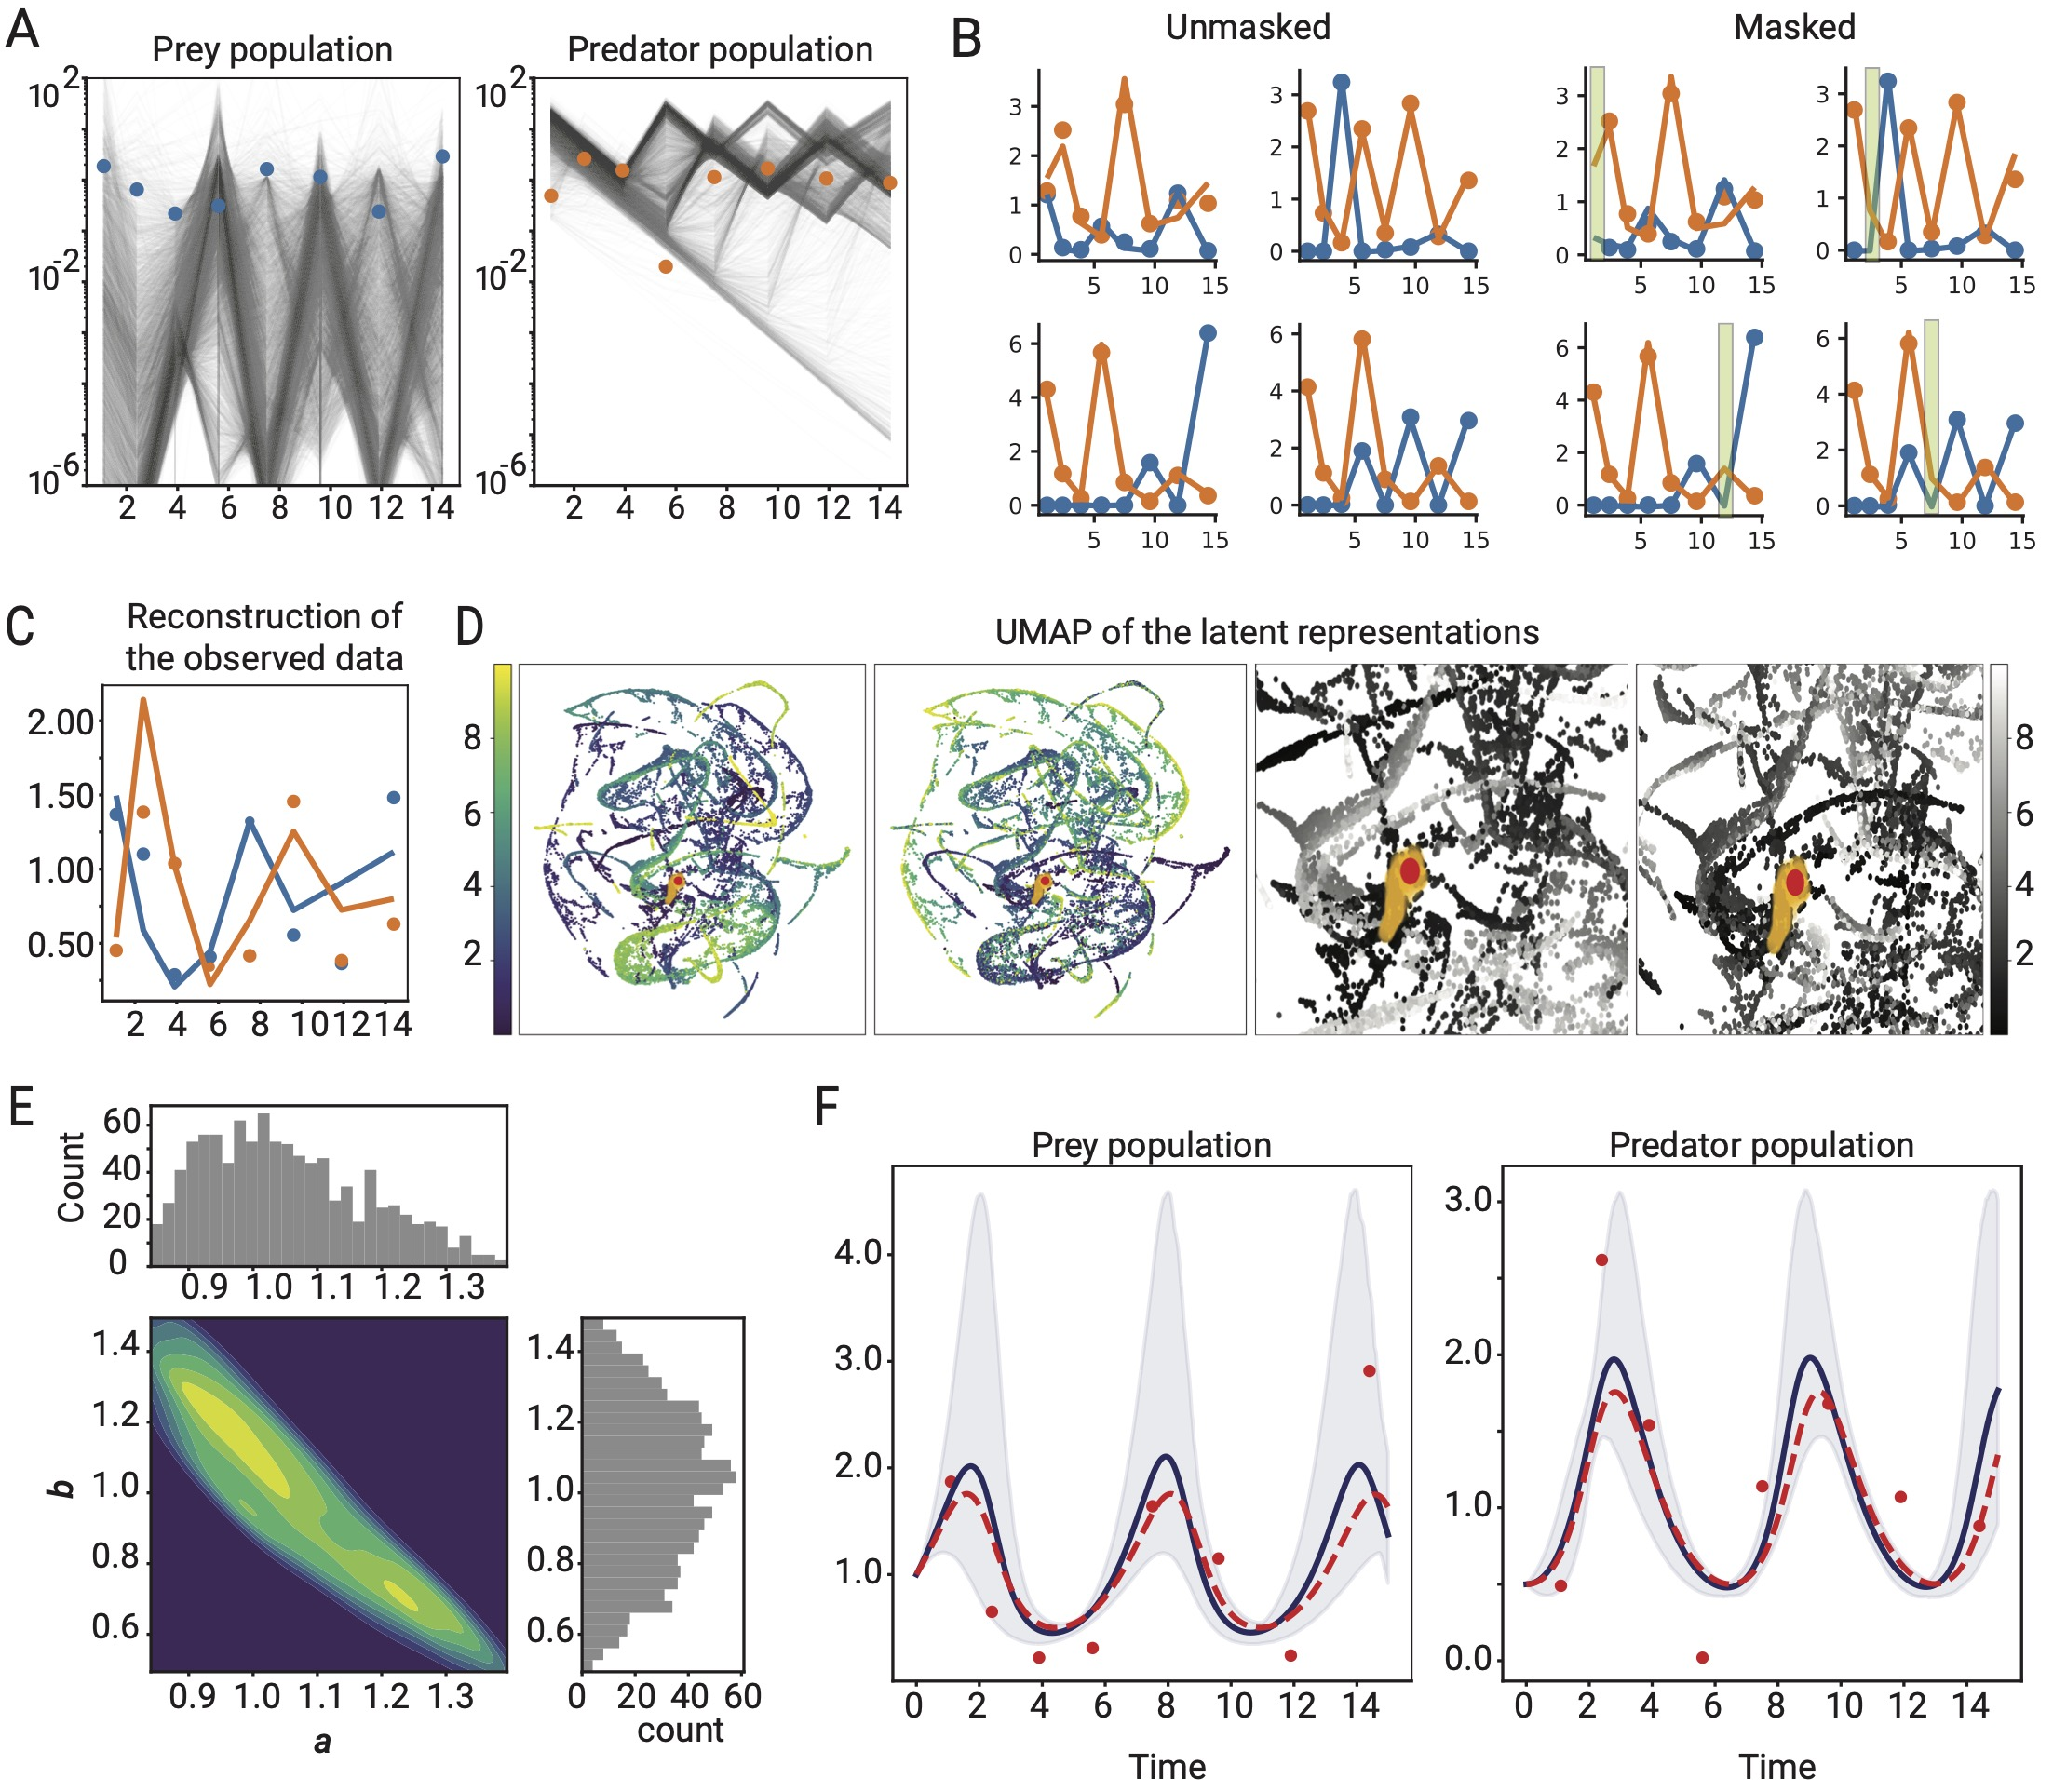
\includegraphics[width=1\linewidth]{figures/figure2.jpeg}
\caption{\textbf{Learning and inferring predator-prey dynamics using VIA-ABC}.
Visualization of the latent representation of simulated and observed data and the final posterior
Density plot of the final iteration of viaABC. The estimated 95\% highest posterior density (HPD) intervals for a and b are [0.9510, 1.1883] and [0.7685, 1.3525], respectively.}
    \label{fig:lv}
\end{figure}

- predictions (including reconstruction?) and posterior surface.
high dense regions around the ground truth -- means its working. 


- Parameter acceptance 

red is gt


\begin{table}[htbp]
\centering
\begin{tabular}{l cccc}
\toprule
Statistics & viaABC & ABC-DRF & ABC-SMC & ABC-SMC-DRF \\
\midrule
$\mathbb{E}$(a) &\textbf{1.0641} & 0.7562 & 1.2912 & 1.1215 \\
Var(a) & \textbf{0.0053} & 0.5953 & 0.1104 & 0.0333 \\
$\mathbb{E}$(b) & 1.0571 & 1.3092 & \textbf{1.0269} & 0.9704 \\
Var(b) & \textbf{0.0299} & 0.3593 & 0.1049 & 0.0313 \\
\bottomrule
\end{tabular}
\caption{Means and variances of marginal posterior distributions for the deterministic Lotka-Volterra model from viaABC, ABC-DRF, ABC-SMC and ABC-SMC-DRF. The best result for each statistic across different algorithms is in bold (E(a), E(b) closest to true values (a, b) = (1, 1), and lowest variance in each statistic). Results are taken from Dinh et al. \citep{dinh2024approximate}.}
\label{tab:lotka_volterra_results} % Add a label for referencing
\end{table}


\subsection*{Characterizing the effects of hyperparameters on VIA-ABC's performance}

\textbf{Masking ratio.} Figure shows the influence of the masking ratio. The ratio of 15\% seems to work well, which is in agreement with the behavior of BERT \citep{devlin2019bert}, whose masking ratio is 15\%. 

\textbf{Decoder design.} In accordance with the original MAE paper, our TSMVAE decoder can be flexible designed, as studied in Table. Table varies the decoder depth and dimension. A sufficiently deep decoder is important for denoising.

\textbf{Data augmentation.} Table studies the influence of different noise level injected used in our TSMVAE pre-training. Our TSMVAE works well using Gaussian noise.  needs to be data dependent and channel dependent.

\textbf{Beta} Table studies the influence of different beta levels used in our TSMVAE pre-training. Based on our study, a beta value of 0.001 



\subsection*{Stochastic Susceptible-Infected-Recovered model}
The stochastic Susceptible-Infected-Recovered (SIR) model is a fundamental framework in epidemiology for capturing the spread of infectious diseases within a population \cite{dd}. Unlike its deterministic counterpart, which employs ordinary differential equations, the stochastic SIR model incorporates intrinsic randomness in disease transmission and recovery, making it particularly suitable for modeling outbreaks in finite populations. The system tracks the evolution of three state variables: $S, I,$ and $R$, representing the number of susceptible, infected, and recovered individuals, respectively. The model dynamics are governed by the following reaction scheme:  
\begin{align*}
S + I &\xrightarrow{\beta} 2I\\
 I &\xrightarrow{\gamma} R
\end{align*}
where $\beta$ denotes the transmission rate per susceptible-infected pair, and $\gamma$ represents the recovery rate of infected individuals. To capture the stochastic nature of infection and recovery events, we employ the Gillespie algorithm \citep{gillespie1977exact}, which simulates the discrete event-driven evolution of the system.\\
In this study, we set $\beta = 2 $ and $ \gamma = 0.5 $ and simulate the epidemic dynamics over a time span of $T = 15$ days, starting from an initial condition of $ (S(0), I(0), R(0)) = (290, 10, 0) $ in a closed population of size $N = 300$. The stochastic trajectories are recorded at thirty-five distinct time points, and to account for observational uncertainty, normally distributed noise $ \epsilon_t \sim \mathcal{N}(0, 1^2) $ is added to each recorded data point. The resulting dataset, denoted as
$s^{\mathrm{obs}} = \{ S_1, I_1, R_1, \dots, S_{35}, I_{35}, R_{35} \} $  
serves as the empirical basis for inference in this study. Since events in the Gillespie algorithm occur at irregular time intervals, we interpolate the simulated trajectories to align their time indices with those of the observed data, ensuring comparability in the inference process.

% \subsection*{Deterministic Marginal Zone B Cell Dynamics}
% PLACEHOLDER \citep{verheijen2020fate}


\textbf{Figure Something}: a) Predicted trajectories of stochastic sir and the observed data points. (b) Final approximate posterior distribution of parameters inferred by the ABC-SMC sampler.

% \subsection{Deterministic Marginal Zone B Cell Dynamics}

% \textbf{Figure Something}: a) Predicted trajectories of marginal bzone. (b) Final approximate posterior distribution of parameters inferred by the ABC-SMC sampler.

% \textbf{Figure Something}: Comparison between 


\section*{Discussion}

In this study, we introduced viaABC, a novel approach for parameter inference in mechanistic models of biological systems. By leveraging the power of variational autoencoders (VAEs) and the principles of approximate Bayesian computation (ABC), viaABC offers a flexible and efficient framework for inferring model parameters from noisy multivariate time series data.
We demonstrated the effectiveness of viaABC on synthetic datasets generated from the Lotka-Volterra model and the stochastic SIR model, showcasing its ability to accurately recover model parameters and capture the underlying dynamics of the systems. The results indicate that viaABC outperforms traditional ABC methods, such as ABC-DRF and ABC-SMC, in terms of parameter estimation accuracy and computational efficiency.

The integration of VAEs allows viaABC to learn meaningful latent representations of the data, enabling it to handle high-dimensional and noisy observations effectively. By encoding the data into a lower-dimensional latent space, viaABC can focus on the essential features of the data while discarding irrelevant noise, leading to improved parameter inference.
The use of a VAE also facilitates the incorporation of prior knowledge about the model parameters, allowing for more informed inference. The ability to leverage pre-trained VAEs further enhances the efficiency of viaABC, as it can initialize the inference process with informative latent representations.

The results of our experiments demonstrate the robustness of viaABC across different datasets and parameter settings. The method's performance is consistent, even in the presence of noise and variability in the data. This highlights its potential for real-world applications in biological systems, where data can be noisy and complex.
The proposed method has several advantages over traditional ABC methods. Firstly, viaABC is computationally efficient, as it can leverage the power of VAEs to learn representations of the data in a lower-dimensional space. This reduces the computational burden associated with simulating large datasets and allows for faster parameter inference. Secondly, viaABC is flexible and adaptable, making it suitable for a wide range of mechanistic models and biological systems. The method can be easily extended to incorporate additional features or modifications, allowing researchers to tailor it to their specific needs.

Finally, viaABC provides a principled framework for parameter inference, combining the strengths of VAEs and ABC. By integrating these two powerful approaches, viaABC offers a comprehensive solution for parameter inference in mechanistic models of biological systems.


\section*{Methods}
\vspace{3mm}

\para{Data generation for the Lotka-Volterra model}

We solved the Lotka-Volterra system and evaluated prey and predator populations  $x(t), y(t)$ at eight distinct time points between \(t = 0\) and \(t = 15\) using parameters $a=b=c=d=1$  and the initial conditions \((x(0), y(0)) = (1, 0.5)\), similar to Toni and Khanh et al~\red{CITE}.
Of note the initial conditions of $(1, 0.5)$ are used for simplicity and do not have any biological meaning.
We further added the Gaussian noise \(\epsilon_t \sim \mathcal{N}(0, 0.5^2)\) to  $x(t), y(t)$evaluated at , by setting \(\theta = (1, 1)\).
This forms our noisy input data $s^{\mathrm{obs}} = \{x_1, y_1, \dots, x_8, y_8\}$ that we use to evaluate VIA-ABC's performance~(\textbf{Figure \ref{fig:lotka-volterra}}).
However, we also validated our approach in a scenario where we inferred all four parameters WE CAN TRY!

We generated a dataset of 50,000 samples from the Lotka-Volterra model, with each sample representing a multivariate time series of length 8.
The parameters \(a\) and \(b\) were sampled uniformly from the range \([0, 10]\).
The generated data was then corrupted with Gaussian noise to simulate real-world observations.

%
%\section{Introduction}
%
%\textbf{Main idea:}
%
%\begin{itemize}[label=$\bullet$]
%\item Train a VAE to generate a latent representation $(Z)$ of data simulated from mechanistic models, in the hope that $Z$ contains model parameters that govern `global' temporal dependencies and latent variables that are `local' to individual data points.
%
%\item Employ an MLP (NN) to recover the learned model parameters.
%
%\item Replace simulated data with observed biological data to infer biological mechanisms.
%
%\end{itemize}
%
%\vspace{6mm}
%
%\textbf{Paper outline:}
%
%\begin{enumerate}[label=\Alph*.]
%    \item Introduction
%    
%    \begin{itemize}
%        \item Background on mechanistic models and their inference. 
%        \begin{itemize}
%            \item \textit{Common problems with mechanistic inference: }
%            \begin{itemize}[label=$\circ$]
%                \item Data and model complexity (e.g. heterogeneity)
%                \item Suited for low dimensional data inference at higher dimensions comes at a cost of non-meaningful and indiscernible parameters
%                \item Inefficient handling of noise in data, etc.
%            \end{itemize}
%        \end{itemize}
%        
%        \item MCMC and variational inference (VI) both can resolve these to some extent, in differential capacity, perhaps.
%        \begin{itemize}
%            \item Why variational inference over MCMC?
%            \item Background on VI  and its application to mechanistic models.
%        \end{itemize}
%    \end{itemize}



%\end{enumerate}

% citations
% note that the .bib file should be in the same directory as the .tex file
% and the .bib file should be named refs.bib
\bibliographystyle{unsrt}
\bibliography{refs}


\end{document}